\chapter{Results}

Results are shown from two machines.

The first machine has a dual-core Intel IvyBridge i7-3520M processor with 12GB
RAM running Debian Jessie/Stretch using g++ 6.1.1.

The second machine has 2 quad-core AMD Opteron 4386 processors with 64GB RAM
running Ubuntu 14.04 LTS using g++ 5.4.0.

Tests are performed on each machine up to twice the number of physical threads;
the maximum number of threads tested are thus 4 and 16. These utilize hyperthreading
to run two simultaneous threads per core, but hyperthreads will not necessarily
provide the same performance as running each thread on its own physical core [cite].



\section{Reduce}
Results shown compare various implementations of a reduce operation of a random
vector of doubles:

\begin{itemize}
 \item ``seq'' is a sequential implementaiton;
 \item ``vec'' is a sequential implementation, but with values always stored in
 vectors (e.g., results of ``reduce'' operations are stored in size-1 vectors).
 This is provided because in order for this method to operate in parallel on
 vectors, the result operations must be itself stored in a ctvector, for
 comparison's sake, tests are performed with the same restriction with a
 std::vector;
 \item ``omp'' is an OpenMP implementation. It uses the maximum number of cores
 available in all cases, so it is also not sensitive to the number of
 threads/cores that are manually selected;
 \item ``avx'' uses a 256-bit AVX instruction to perform the addition of 4 doubles
 simultaneously until only 4 values remain, and then uses more avx instructions
 to sum the resulting values. Thus, the speedup of this implementation can be
 compared directly to other implementations when using 4 concurrent threads;
 \item ``async`` is a C++11-style parallel implementation using the C++ std::async
 feature to launch threads, each of which are given a fraction of the list equal
 to the inverse of the total number of threads.
\end{itemize}

\begin{figure}[!h]
\centering
    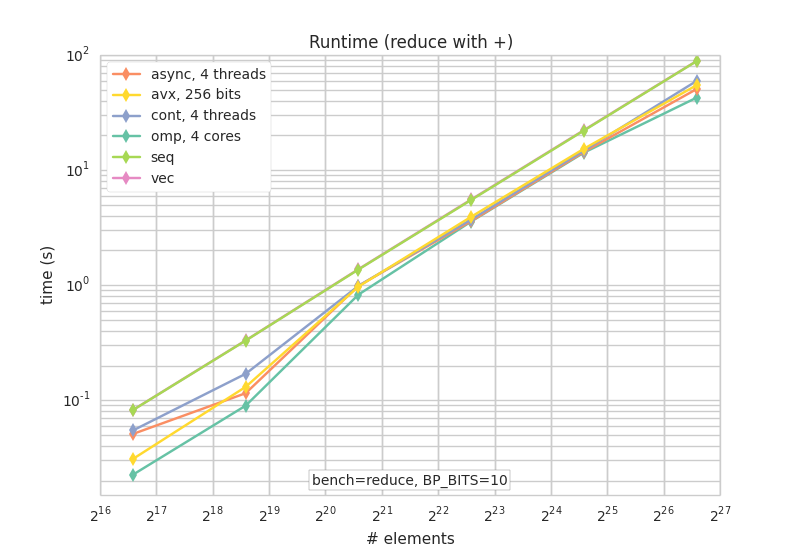
\includegraphics[width=0.5\textwidth]{graphs/cont-reduce_sz-vs-time.png}
\end{figure}
\begin{figure}[!h]
\centering
    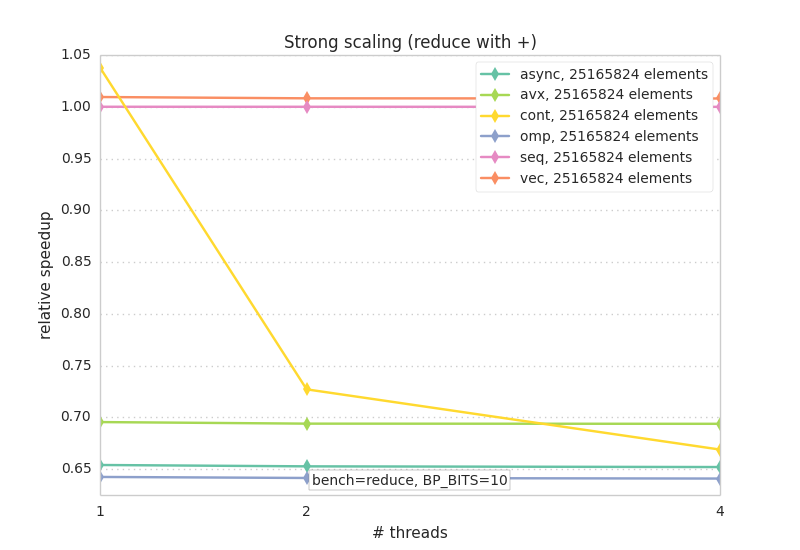
\includegraphics[width=0.5\textwidth]{graphs/cont-reduce-large_procs-vs-speedup.png}
\end{figure}

\section{Foreach}
Results show strong and weak scaling for the contentious library performing a
foreach operation on a random vector of doubles. For comparison, the results
show the runtime of a serial implementation as well.

\section{Heat}
Results show strong and weak scaling for the contentious library using a
1st-order scheme to compute the heat equation framed as a Boundary-Value
Problem.

\begin{comment}
With optimization turned on vec behaves a lot like seq. Without
optimization, vec is a lot slower. All these benchmarks use optimization flags,
so the results are almost identical between seq and veche "async"
implementation uses C++ threads with the async
\end{comment}
